\section{Theory}
	\subsection{Data structure}
The presidential election data used in this project was downloaded from GeoDa[2]. The underlying information in the dependant variables, constructing the design matrix, are all drawn from the years between 2007 and 2014. They represent sociological aspects such as education, wealth, ethnicity, population density among others. The response variable is the percentage outcome for the democrats and republicans. The response variable was in this work modified from percentage outcome into ones and zeros with a 50\% cut-off. Democratic counties became ones. The problem can now be death with as supervised learning and classification.
\\
\par  
As mentioned above, the dependent variables together construct the design matrix. The design matrix has the dimensions (3108, 51), 3108 counties and 51 variables. There are two independent variables, namely the political outcome for each election, 2012 and 2016. The independent variables are each a binary vector with the dimensions (3108, 1). After a reshuffle of the rows, or counties, 75\% of the rows are used for training and cross validating a model, and 25\% are left for testing on unseen data on the 2012 election. Then the model is applied on the same design matrix without splitting and reshuffling to make predictions on the 2016 election.
\\
\par
Since most machine learning algorithms rely on euclidean distances they do not perform well when the data is scaled differently. In this case the data is both large and low in numerical measurements, with the addition of percentage variables. Therefore, we transform the data by Scikit learn's preprocessing function 'StandardScaler'. The function subtracts the column mean and divide by the column standard deviation for each column [3]. 
\\
\par
	\subsection{Cross validation}
The model is first trained for all the data and model statistics are calculated. Then the model is validated and tested to assure the quality of the model. The validation technique used to validate the different models is cross validation. Cross validation is widely used when the data set is small or finding the difference between the true value and the prediction for a single or a sample of observations. When the data set is small, the resulting model is more sensitive to an arbitrary splitting of the data into training data and test data. The split could be leaving out important data from the training part. Another common validation technique is bootstrap. 
\\
\par

\begin{figure}[H]
\centering
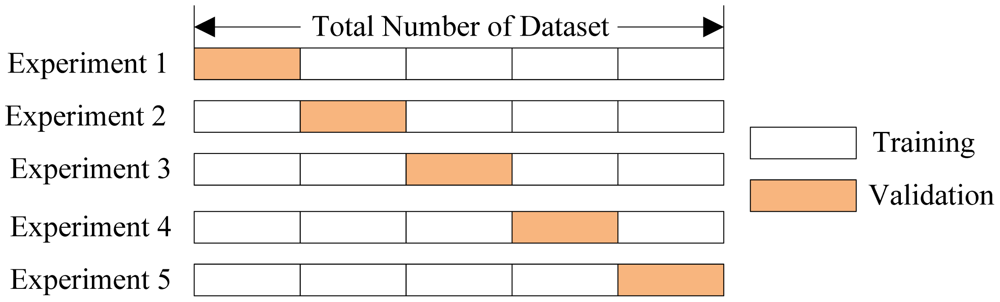
\includegraphics[scale=0.3]{pictures/Cross_validation}
\caption{Cross validation explained graphically. The idea of cross validation. A small part of the data is used for training. The other larger part for testing/validation. Then another experiment and the test data changes and thus, so does the training data. In the end all data was test once but only once.}
\end{figure}

	\subsection{Logistic regression}
\setlength{\parindent}{0cm}
A popular binary classification method is the logistic regression, especially among statisticians. This is because it's a more statistical approach to a classification problem than support vector machines or decision trees. There’s no analytic expression for the coefficients, so these must be calculated numerically. How the mathematical problem is dealt with is briefly described below. 
\\
\par 

\begin{figure}[H]
\centering
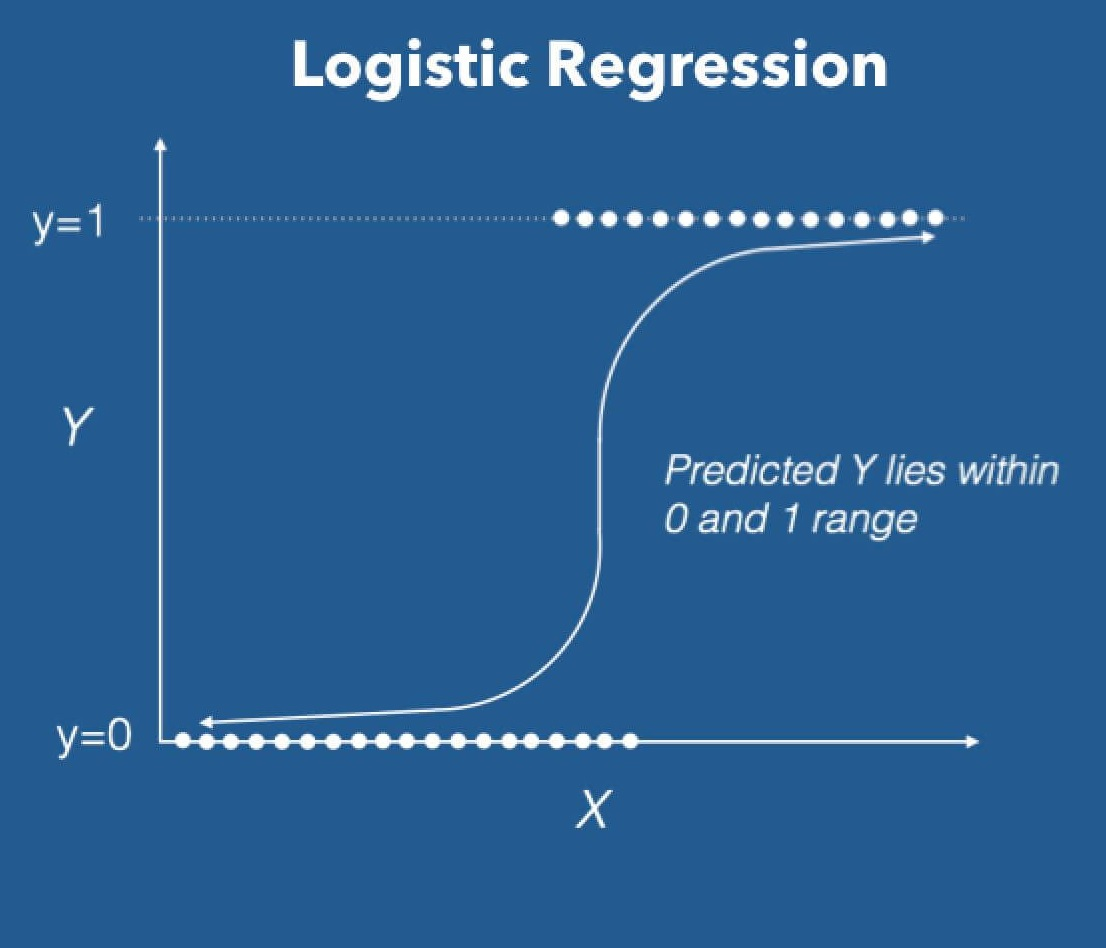
\includegraphics[scale=0.2]{pictures/LogReg}
\caption{Logistic regression displayed graphically}
\end{figure}

The logistic function is called the Logit or the Sigmoid function (see below). It returns a value or interpreted as a probability between 0 and 1. $\beta$ is the wanted coefficients and $x_i$ is an observation. The function tries to map the product of these two to either 0 or 1, but some input values will give an output value in-between. This is where the the function sharply rises. At this range of input values, the observations do not belong to a clear category.    
\begin{equation}
p(\beta x_i)=\frac{1}{1+exp^{-\beta x_i}}
\end{equation}
\par

Moving on to deriving the cost function. The given probabilities could be either 1 or 0.
\begin{equation}
p(y_i = 1\vert x_i,\hat{\beta}) = \frac{1}{1+exp^{-\hat{\beta x_i}}}
\end{equation}
\\
\begin{equation}
p(y_i=0\vert x_i,\hat{\beta})=1-\frac{1}{1+exp^{-\hat{\beta}x_i}}
\end{equation}
\\
\par

To obtain a cost function, define the total likelihood for all possible outcomes from a data set D = {($y_i,x_i$)}, with the binary labels $y_i \in$ {0,1} and where the data points are drawn independently, and then apply the Maximum Likelihood Estimation (MLE), i.e., maximizing the probability of seeing the observed data and approximating the likelihood in terms of the product of the individual probabilities of a specific outcome $y_i$. 
\begin{equation}
P(D\vert \hat{\beta})=\prod_{i=1}^{n} [p(y_i=1\vert x_i,\hat{\beta})]^{y_i} 
[1-p(y_i=1\vert x_i,\hat{\beta})]^{1-y_i} 
\end{equation}
\\
\par

From the MLE, then the logistic regression has the following cost function. 
\begin{equation}
C(\hat{\beta})=\sum_{i=1}^{n}(y_i log[p(y_i=1\vert x_i,\hat{\beta})]
+(1-y_i)log[1-p(y_i=1\vert x_i,\hat{\beta})])
\end{equation}
\\
\par
By defining a vector $\hat{y}$ with n elements $y_i$, an n×p matrix $\hat{X}$ which contains the $x_i$ values and a vector $\hat{p}$ of fitted probabilities $p(y_i \vert x_i,\hat{\beta})$, the first and second derivative of the cost function can be rewritten in a more compact way. 
\begin{equation}
\frac{\partial C(\hat{\beta})}{\partial\hat{\beta})}=-\hat{X}^T(\hat{y}-\hat{p})
\end{equation}
\\
\begin{equation}
\frac{\partial^2 C(\hat{\beta})}{\partial^2\hat{\beta}}=\hat{X}^T\hat{W}\hat{X}
\end{equation}
$\hat{W}$ is a diagonal matrix with the elements $p(y_i=1\vert x_i,\hat{\beta})
(1-p(y_i=1\vert x_i,\hat{\beta}))$
\\
\par

To find the minimum of the cost function, several approaches are possible. One possibility is the multivariate version of the Newton-Raphson's method. Newton-Raphson's method tries to find a root of a function f(x). 
\begin{equation}
x^{(k+1)}=x^{(k)}-J_f(x^{(k)})^{-1}f(x^{(k)}) 
\end{equation}
where J is the Jacobian of f. A matrix of all first-order partial derivatives of the function.
\\
\par

The problem will have to be redefined as finding where the gradient of the function is equal to zero, $\nabla f(x)=0$. Because we seek the roots of the derivative of the cost function.
\begin{equation}
x^{(k+1)}=x^{(k)}-(H_f(x^{(k)}))^{-1}\nabla f(x^{(k)}) 
\end{equation}
where H is the Hessian of f. A square matrix of second-order partial derivatives of the function.
\\
\par
For logistic regression, Newton-Raphson's method will then look the following way. 
\begin{equation}
\hat{\beta}^{new}=\hat{\beta}^{old}-(\hat{X}^T\hat{W}\hat{X})^{-1}
(\hat{X}^T(\hat{y}-\hat{p}))
\end{equation}
$\hat{\beta}^{old}$ must be randomly initialized to start the iteration. $\hat{p}$ is the output from Sigmoid($\hat{\beta}X$).The iteration continues until the some criteria is reached, like the change in $\hat{\beta}$ is acceptable small.[4]   
\\
\par

Computing the inverse of the Hessian, $\hat{X}^T\hat{W}\hat{X}^{-1}$, could be computationally expensive. Therefore, in larger datasets a gradient descent method is used instead. 
In practice, it means the Hessian is replaced by a scalar, also called a learning rate. Newton-Raphson's method could in addition to the second derivative also include a learning rate, but without it's known as "pure Newton". The function is convex, so Newton-Raphson's method or any gradient descent method will always converge to the minimum, a global minimum. [5]
\\
\par
	\subsection{Neural networks}
\begin{figure}[H]
\centering
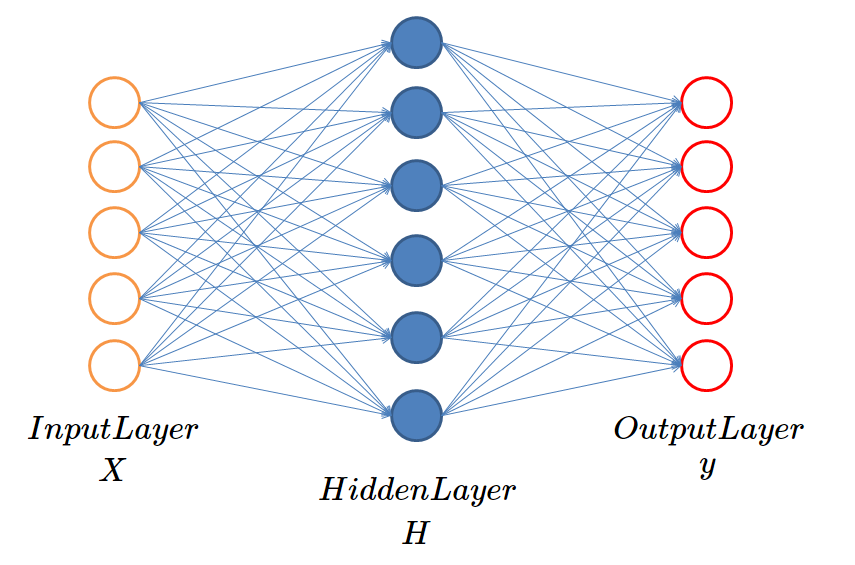
\includegraphics[scale=0.4]{pictures/NN_schematic.png} 
\caption{Neural network architecture layout}
\end{figure}
{\small Source: \url{https://chunml.github.io/ChunML.github.io/} \par  \url{project/Creating-Text-Generator-Using-Recurrent-Neural-Network/}}
\\
\par
A neural network is constructed as shown above. In that case, the output layer contains more than one output, as it could be any desired number. One hidden layer is added, constructing a net of weights (blue lines) and biases. Additional hidden layers can be included. Each hidden layer can be assigned arbitrary many neurons (the blue circles). The idea is sprung from the logistic regression extended into a more complex configuration of interconnected elements that processes the information dynamically. It's also influenced by neuroscience, and how the human brain works. Further break down of the concept is as follows, with the encapsulated iteration process in mind:[6] 
\\
\par
First, we choose the cross entropy function as our cost function, defined in Eq[6].
\\
\par
\textbf{Forward phase}\\
Weights and biases are often created randomly and normally distributed. The net input value (Z) is then calculated as:

    \begin{equation}
       Z =   X \bullet W + b
    \end{equation}
Noted is that the calculations now take place as nestled matrices, where the matrix \textbf{$W$} represent all weights on both sides of a calculated layer, hence have the size (2,).\\
\par

Z is then activated by chosen activation function for the interaction between the input layer and the hidden layer, and similarly by the hidden and output layer.

    \begin{equation}
       a(Z)
    \end{equation}

\textbf{Backpropagation phase}\\

An error calculation is made by use of the cost function, which is denoted [$\delta_3$]. Next step is to update the weights and biases such that the error between the target and output decreases towards a global minima. This step is the essence of a neural network and is often noted as the backpropagation algorithm, which evaluate the error and uses partial gradients to pass the necessary adjustments back into the system. For cross entropy as the choice of cost function and Sigmoid as the activation functions, the backpropagation algorithm is implemented as below:[7]
\\
\par
    \begin{equation}
       \delta_3 = (yp-y) 
    \end{equation}
    \begin{equation}
       \delta_2 = \delta_3 \bullet W{_2^T} * (a(Z_1))' 
    \end{equation}
    \begin{equation}
       \frac{\partial C}{\partial W_2}  = a(Z){_2^T} \bullet \delta_3
    \end{equation}
    \begin{equation}
       \frac{\partial C}{\partial b_2}  = sum(\delta_3)
    \end{equation}
    \begin{equation}
       \frac{\partial C}{\partial W_1}  = X^T \bullet \delta_2
    \end{equation}
    \begin{equation}
       \frac{\partial C}{\partial b_1}  = sum(\delta_2)
    \end{equation}
Layers are representative by (1,2,3) = (I,$H_1$,O) such that the recipe can be extended if additional hidden layers are added, as (1,2,3,4) = (I,$H_1$,$H_2$,O). Note that if the cost function or the activation function are changed, one would have to derive $\delta_3$ from scratch.
\\
\par

There must be highlighted that the neural network are prone to some parameters that governs entirely how well the model will preforms.[7]
\\
\par
\textbf{Learning rate}\\
This is a hyperparameter that controls how much the weights and biases will adjust due to the gradient of the cost function. A small value could be described as taking small, but accurate steps towards the minimum. For a large value, the path towards the minimum would be rough. To large and there is a probability of never reaching the precise minima, while to low may be stuck at a plateau. It also affects the computational time, a large learning rate would decrease the computational time and vice verse.
\\
\par
\textbf{Regularization term}\\
By applying a regularization term, the weights and biases (or coefficients for the linear case) is basically programmed to be small, with the assumption that a lower variance between them would represent a simpler model, hence it is a way of avoiding overfitting.
\\
\par
\textbf{Epochs}\\
Denotes how many times a training set is run through the neural network, both forward and backward. By increasing the number of epochs one would expect the model to obtain optimal weights and biases, only running it once would underfit the model.
\\
\par
\textbf{Batch size}\\
Included in the SGD method, the training data is divided into smaller batches which run separately through the neural network. So instead of running the whole training set in one epoch, all batches runs once for one epoch. This allows us to run larger datasets. Optimal batch size is discussed, but the size will effect the convergence of the gradient. Generally a small batch size in the range of 32-512 is preferred.
\\
\par
\textbf{Layers and neurons}\\
Increasing the number of neurons or layers also increase the networks ability to learn detailed parts of the data, so for a complex situation more neurons and / or layers would be beneficial. This can be adjusted along the way, by doing a grid search for different numbers and compare the final score. The configuration also have impact on the proper choice of activation function.
\\
\par
\textbf{Activation function}\\
The choice of activation function will have impact on how the model preform as it transform the values into different domains. They may have steeper gradients and lower computational time, or be able to avoid vanishing gradients allowing deeper nets, or decrease the probability of exploding cost functions. For a network with multiple layers, one could use different functions for each layer. Without the activation functions, neural networks wouldn't preform as well as they do.
\\
\par
The above theory is nicely implemented in the package Tensorflow with Keras. Constructing a neural network with the package can be described with a few lines:

\begin{verbatim}
  # Set up a sequential neural network
  clf = tensorflow.keras.Sequential()
  # Adding a hidden layer and a output layer
  clf.add(tensorflow.keras.layers.Dense(...)
  clf.add(tensorflow.keras.layers.Dense(...)
  # Specify a gradient descent method
  sgd = tensorflow.keras.optimizers.SGD(...)
  # Compile model
  clf.compile(optimizer=..loss=..metrics=..)
  # Fit the model
  clf.fit(X,y,epochs=..batch_size..) 
\end{verbatim}

	\subsection{Support vector machines}
This is a machine learning method that is broadly used in classification problems, but it could just as well be used for regression problems. It relies on supervised data to construct a decision boundary that divides classes in space. The advantage of the algorithm lies partly in the support vectors, marked as dotted lines in figure[5]. The optimal decision boundary (red line) is obtained by maximizing the gap between the support vectors. This feature is highly appreciable when dealing with classes that are difficult to separate. And further advantage is gained by analyzing data in higher dimensions.[8]
\\
\par
\begin{figure}[H]
\centering
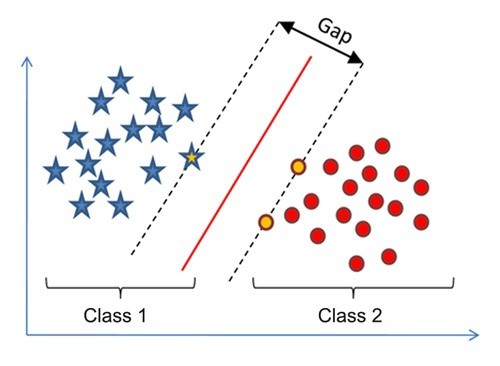
\includegraphics[scale=0.4]{pictures/svm_hyper.jpg} 
\caption{Visualized SVM concept}
\end{figure}

The decision boundary and support vectors are here described by:
\begin{equation}
	y = w^Tx+b=0 \qquad , \qquad y = w^Tx+b=\pm1
\end{equation}
Where [w] is the normal vector to the decision boundary, [b] is the bias. The maximal margin, or gap in figure[5] is defined as:
\begin{equation}
	max_w \frac{2}{||w||} \qquad or \  equivalently \qquad min_w||w||^2
\end{equation}
\textbf{Cost function:}\\
Mentioned margin is to be optimized. But first we introduce a slack variable [$\xi$], which for [$\ \xi \geq ||w||\ $]  a point is misclassified and for [$\  0 < \xi \leq ||w||\ $] a point is located within the margin. This is added as a term which operate as a margin softener, simply allowing for some mistakes, we have:
\begin{equation}
	min_w||w||^2 + C\sum_{i=1}^{m} \xi_i \quad constrained \ to \quad y_i*f(x_i) \geq 1 - \xi_i
\end{equation}
C is the regularization parameter that regulates how much we value the mistakes and [$x_i$] is the support vectors. By including [$\xi_i \geq 0$] in the constraint, we can write the constraint and optimization function respectively as:
\begin{equation}
	[\ y_i*f(x_i) \geq 1 - \xi_i\ ] \rightarrow [\ \xi_i = max(0,1-y_i*f(x_i))\ ]
\end{equation}
\begin{equation}
	min_w||w||^2 + C\sum_{i=1}^{m} max(0,1-y_i*f(x_i))
\end{equation}
Where [$\ f(x_i)=w^Tx_i+b\ $]. The summation term is denoted the hinge loss function, illustrated in figure[6]. 
\begin{figure}[H]
\centering
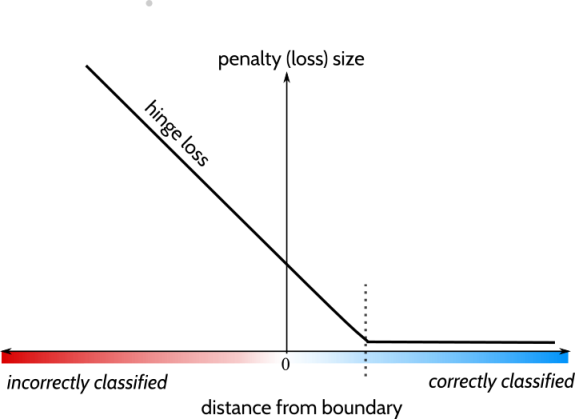
\includegraphics[scale=1.2]{pictures/hinge.png} 
\caption{The hinge loss function}
\end{figure}
Since this a non-smooth function, it's needed to interpret it as a piece-wise function in order to minimize it. We can denote the term inside the summation as: [$\ max(0,1-y_i*f(x_i)) = L(x_i,y_i,w)\ $], by observing the two possibilities:
\begin{equation}
	\frac{\partial(L)}{\partial(w)}=-y_ix_i\ \quad , \quad \frac{\partial(L)}{\partial(w)}=0
\end{equation}

Further, we take use of the Lagrange method and define $\lambda = 2/(mC)$. We can now write the cost function to minimize as:
\begin{equation}
	Cost(w) = \frac{1}{m}\sum_{i=1}^m(\ \frac{\lambda}{2}||w||^2+L(x_i,y_i,w)\ )
\end{equation}

\textbf{Kernel trick}\\
By transforming the above primal form into dual form, the advantage of using the kernel-trick become available. The trick essentially transform a non-separable space into a separable, allowing us to obtain a decision boundary.
\begin{figure}[H]
\centering
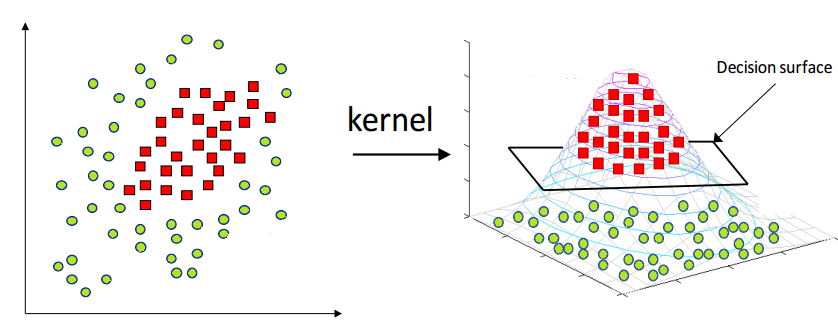
\includegraphics[scale=0.4]{pictures/kernel.png}
\caption{Kernel trick visualized} 
\end{figure}

This is done by observing that the solution [w] can be expressed as a linear combination of the data:
\begin{equation}
	w = \sum_{k=1}^m = \lambda_k,y_k,x_k
\end{equation}
This is then substituted into $f(x_i)$ and the defined cost function, leading to a optimization problem over $\lambda$ instead of $w$, with the following decision function:
\begin{equation}
	f(x) = \sum_{i=1}^m \lambda_iy_iK(x_i,x)+b
\end{equation}
And the optimization function follows as:
\begin{equation}
	max_{(\lambda_i \geq 0)} \ \  \lambda_i - \frac{1}{2}\sum_{kj} \lambda_k\lambda_jy_ky_jK(x_k,x_j)\ for\ [ 0 \geq \lambda \geq C]\  and\  \sum_{i=1}^m \lambda_iy_i = 0
\end{equation}
Finally, the kernel trick can be applied by inserting chosen kernel function suitable for the specific classification problem. A few commonly functions are:
\\
\par
\qquad\textit{Linear}
 \begin{equation}
 K(x_i,x) = x^Tx_i
 \end{equation}
\par
\qquad\textit{Polynomial}
 \begin{equation}
 K(x_i,x) = (x^Tx_i + \gamma)^d
 \end{equation}
\par
\qquad\textit{Radial basis}
 \begin{equation}
 K(x_i,x) = e^{-\gamma||x-x_i||^2}
 \end{equation}
\par

\textbf{Parameters:}\\
For being able to obtain the most efficient model of data, one need to tune some parameters. There is no golden rule, the tuning must be done by consideration for each applied situation. This is usually handled by doing a cross validation search. In addition to the parameters described below the different kernel functions also govern the final results, hence experimenting with those is also recommended.[9]
\\
\par
\textit{C}\\
The parameter that governs the sensitivity of correct classifications. It's essentially a trade-off between the amount of misclassifications on training data and the maximization of the margin between the support vectors. For larger values of C only smaller margins would be allowed and for smaller values the margins would be larger and hence the decision boundary would be simpler, at the expense of accuracy. For $C = \infty$ the margin is denoted hard and do now allow any misclassifications. C is simply the regularization factor for SVM. 
\\
\par
$\gamma$\\
This parameter is part of the kernel function and vary the dependence on whether the algorithm will construct a decision boundary with high consideration of points in its neighbourhood, or not. A low value would loosely fit the data, hence under-fitting it with a less complex boundary, and vice verse for a high gamma value.
\\
\par

The above theory is easily implemented by a two-liner in Scikit learn:

\begin{verbatim}
  # Set up Support Vector Machine
  clf = SVC(C=..,kernel=..,gamma=..)
  # Fit the model
  clf.fit(X,y)
\end{verbatim}